\begin{appendices} 
\chapter{Árbol de Problemas}
\label{anexo1}
\begin{figure}[h]
	\begin{center}
		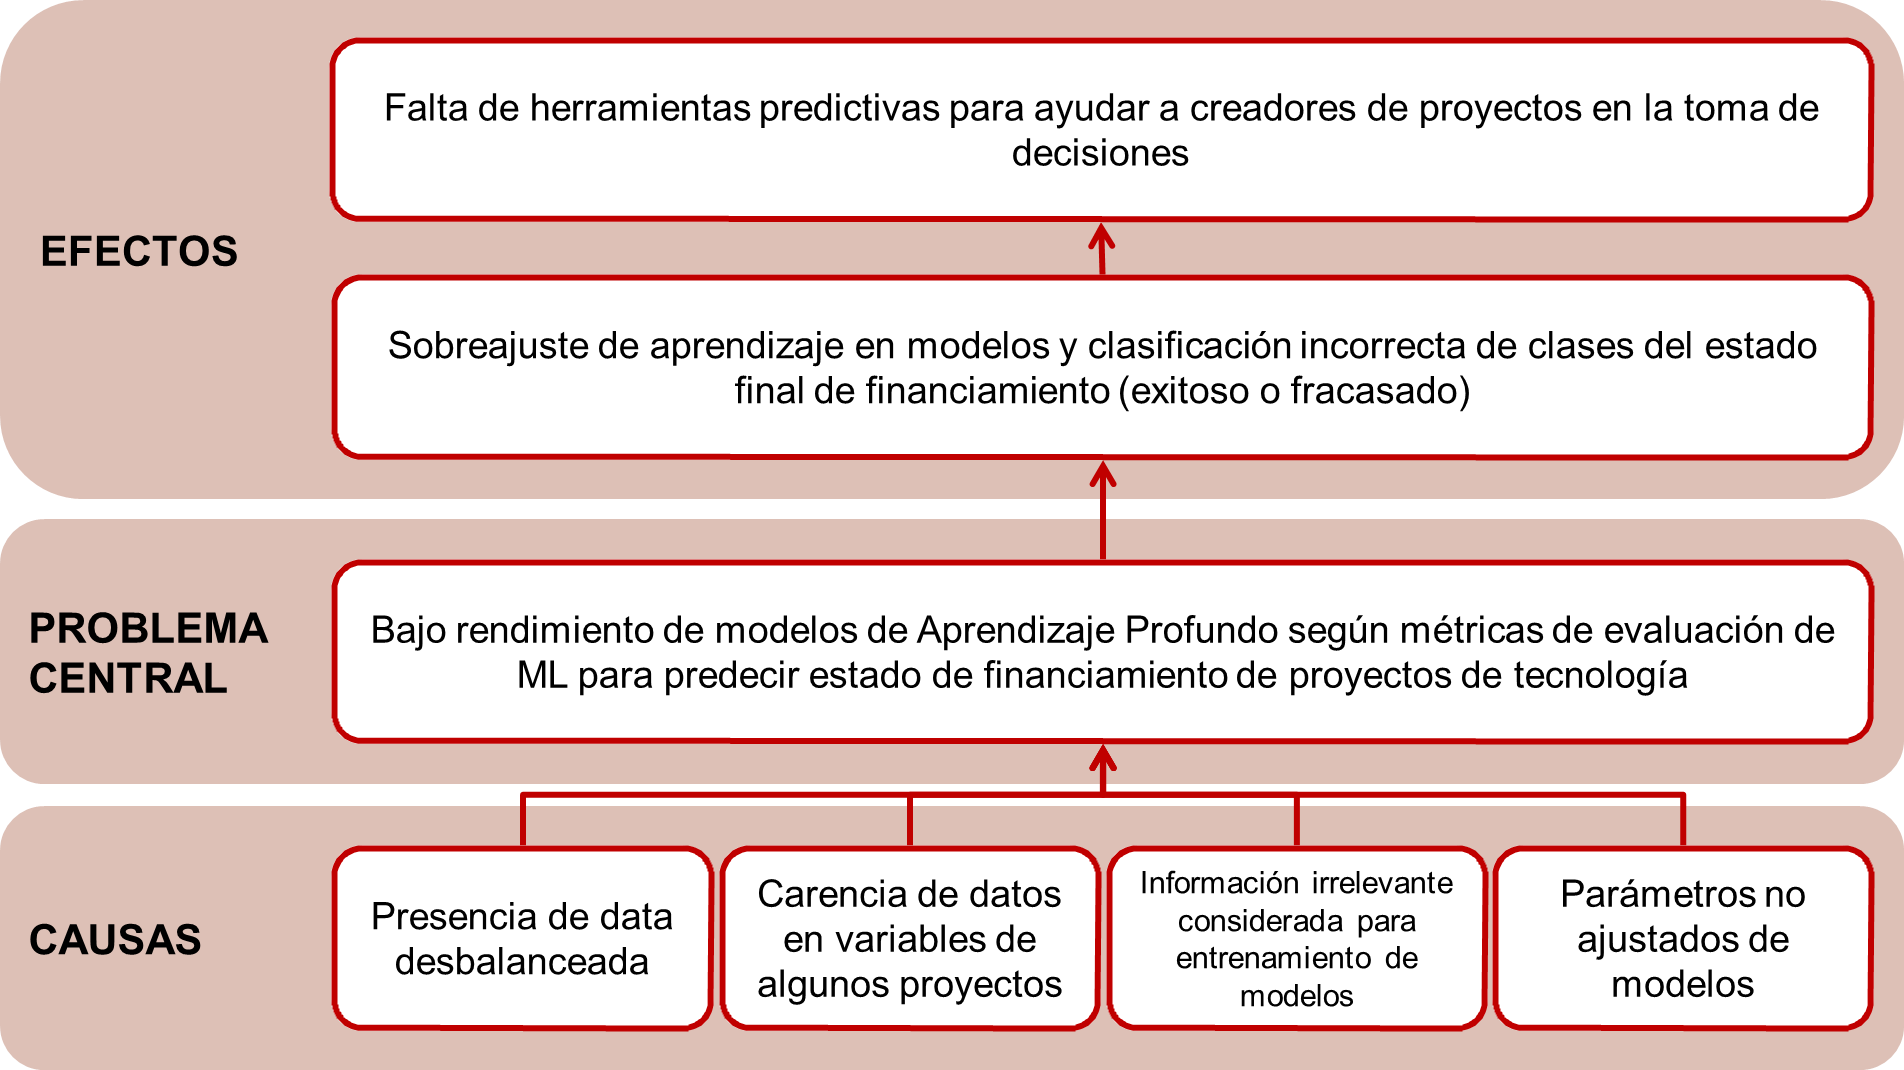
\includegraphics[width=1.0\textwidth]{anexos/arbol_problemas.jpg}
		%\caption{Fuente: Elaboración propia}
	\end{center}
\end{figure}

\chapter{Árbol de Objetivos}
\label{anexo2}
\begin{figure}[h]
	\begin{center}
		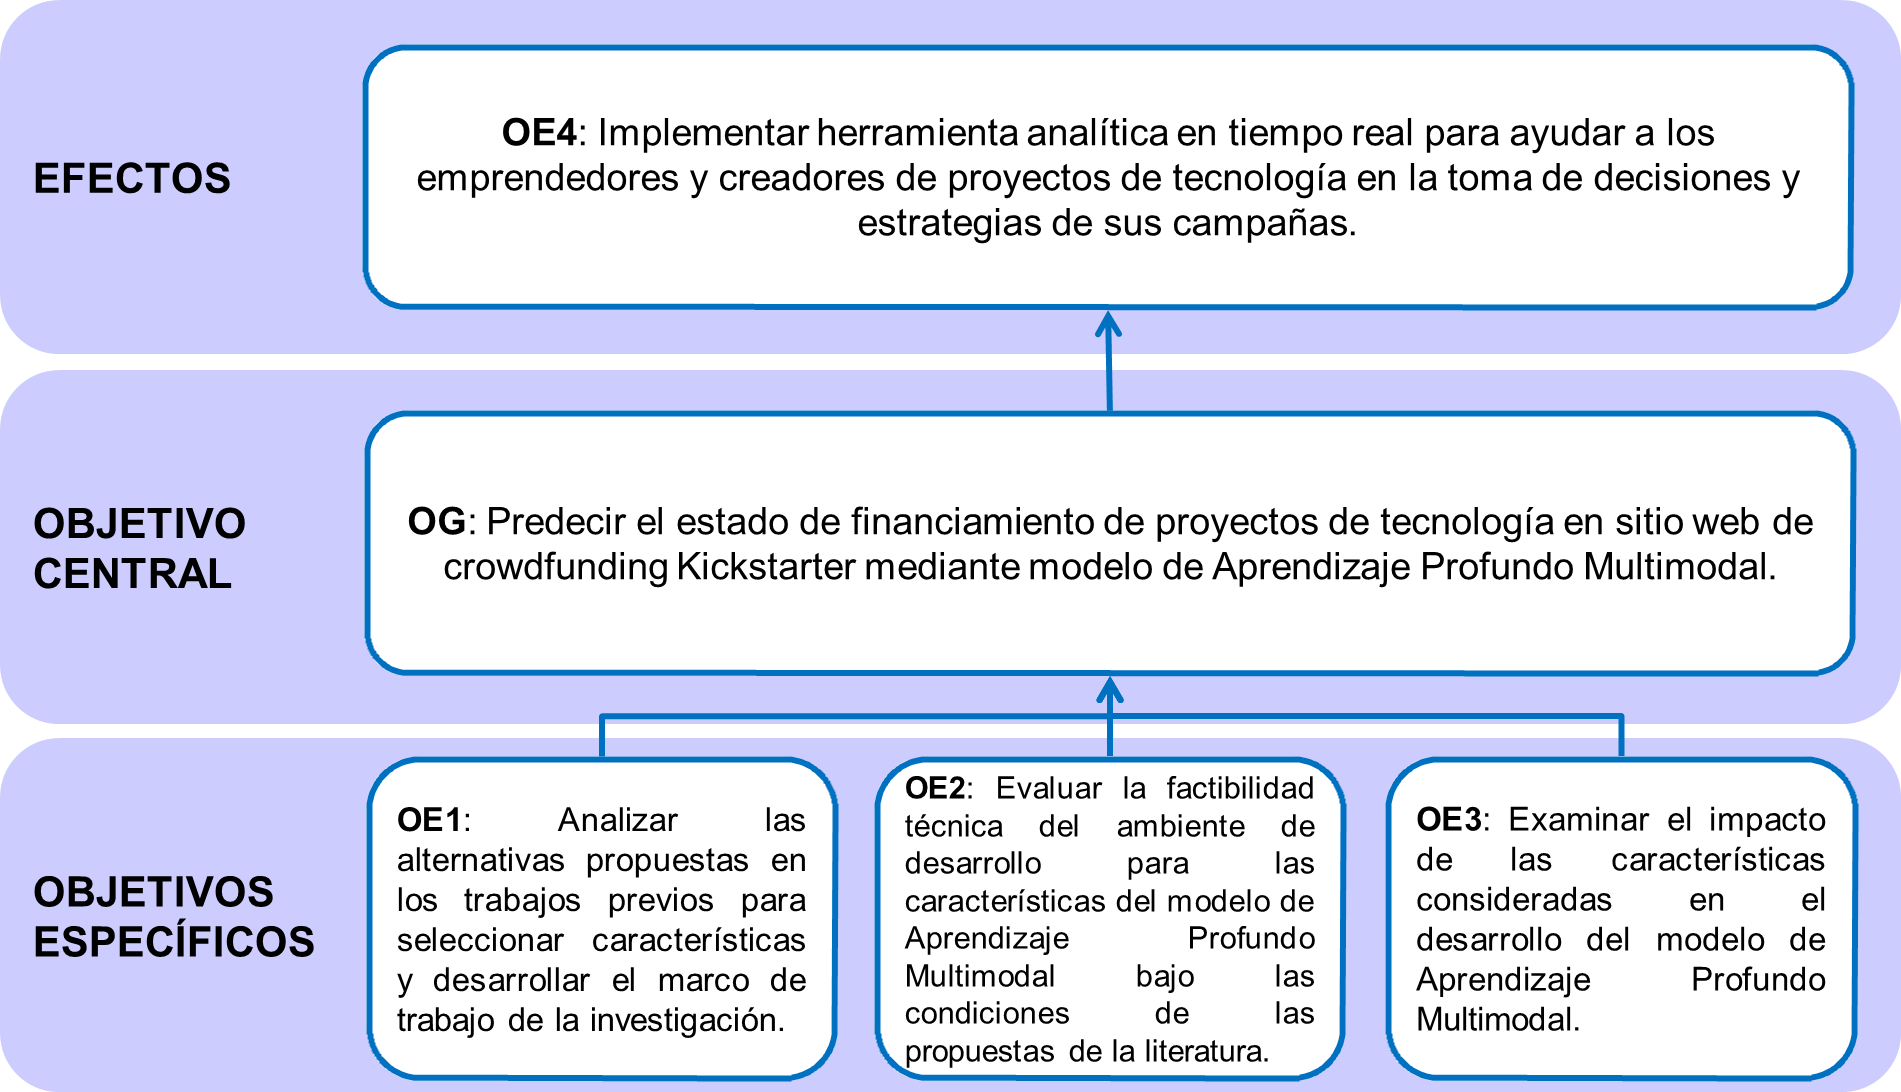
\includegraphics[width=1.0\textwidth]{anexos/arbol_objetivos.jpg}
		%\caption{Fuente: Elaboración propia}
	\end{center}
\end{figure}


\chapter{Matriz de Consistencia}
\label{anexo3}
\begin{table}[h!]
	\centering
	\small
	\begin{tabular}{ |m{5cm}|m{5cm}|m{5cm}|  }
		\hline
		\rowcolor{bluejean}
		\Centering \color{white}{PROBLEMAS}& \Centering \color{white}{OBJETIVOS}& \Centering \color{white}{HIPÓTESIS}\\
		\hline
		\rowcolor{turq}
		\Centering Problema General& \Centering Objetivo General & \Centering Hipótesis General \\
		\hline
		{\ProblemaGeneral} & { \ObjetivoGeneral} & {\HipotesisGeneral} \\
		\hline
		\rowcolor{turq}
		\Centering Problemas Específicos& \Centering Objetivos Específicos & \Centering Hipótesis Específicas \\
		\hline
		{\Pbone} & {\Objone} & {\Hone} \\
		\hline
		{\Pbtwo} & {\Objtwo} & {\Htwo} \\
		\hline
		{\Pbthree} & {\Objthree} & {\Hthree} \\
		\hline
		{\Pbfour} & {\Objfour} & {\Hfour} \\
		\hline
		{\Pbfive} & {\Objfive} & {\Hfive} \\
		\hline
	\end{tabular}
	%\caption{Fuente: Elaboración propia}
\end{table}

\end{appendices} 